\section{Domain Randomization}

Domain Randomization (DR) ist eine weitere Methodik die Realitätslücke zwischen dem Simulator und der echten Welt zu schließen, in dem die Simulation vielfach variiert wird während des Trainingsprozesses. \footcite[Vgl.][S. 3]{Bharadhwaj.2019}
Im Gegensatz zur Systemidentifikation, als Prozess die Parameter bestmöglich an ein physisches System anzupassen, ermöglicht DR einen geringeren Zeitaufwand und geringere Fehleranfälligkeit. \footcite[Vgl.][S. 1]{Tobin.2017}
Teilweise kann durch diesen Ansatz die Diskrepanz soweit geschlossen werden, dass es eine Datensammlung in der echten Welt nicht weiter bedarf. \footcite[Vgl.][S. 2]{Molchanov.2019}
Anhand von Komponenten der Simulationsumgebung lässt sich DR in visuelle und dynamische Randomisierung unterteilen. \footcite[Vgl.][S. 5]{Zhao.2020}
Weitere Methoden die Realitätslücke zu verkleinern sind progressive Netzwerke, inverse Dynamikmodelle und bayessche Methoden. \footcite[Vgl.][S. 2]{Chen.2021}

\subsection{Das Prinzip hinter der Randomisierung von Simulationsumgebungen}

DR verfolgt den Ansatz eine hohe Anzahl an Simulationsumgebungen mit randomisierten Eigenschaften zu erzeugen, in welchen die Strategie dahin optimiert wird, in allen Umgebungen ihr Ziel bestmöglich zu erfüllen. \footcite[Vgl.][S. 1]{Hsu.2023}
Durch das Aussetzen des Agenten gegenüber einer Vielzahl von Umgebungen, wird das Ziel verfolgt den Agenten direkt in die physische Welt übertragen zu können, unter der gleichzeitigen Erwartung einer guten Leistung. \footcite[Vgl.][S. 2]{Chen.2021}
Diese Erwartung resultiert aus der Hypothese, dass unter genug Variabilität die echte Welt lediglich eine bereits trainierte Variation darstellt. \footcite[Vgl.][S. 1]{Tobin.2017}
Dieses Prinzip kann auch der Abbildung fünf entnommen werden, in welcher das physische System im Bereich der Randomisierung der Simulation liegt. 

\begin{figure}[htb]
    \centering
    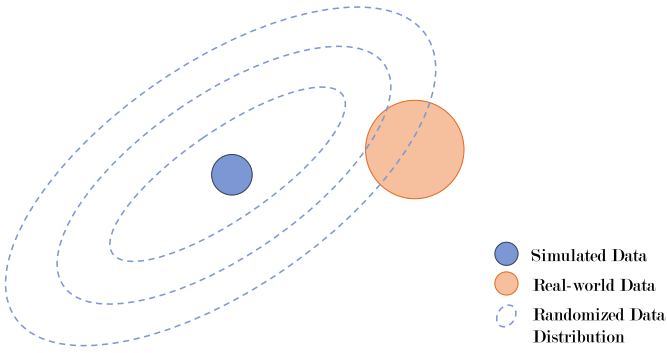
\includegraphics[height=4cm]{lib/graphics/Domain_randomization.png}
    \caption[Intuition hinter dem Paradigma von DR]{Intuition hinter dem Paradigma von DR\footnotemark}
    \label{abb:Domain_randomization}
\end{figure}
\footnotetext{Enthalten in: \cite[][S. 6]{Zhao.2020}}

\subsection{Anwendung von Randomisierung der Simulationsumgebung}

Die Anwendung von DR beginnt nach der Erstellung einer möglichst realen Simulation zum Sicherstellen, dass spätere Variation die wirkliche Welt abbilden können. \footcite[Vgl.][S. 4]{Chen.2021}
Anschließend kann die Randomisierung verschiedener Aspekte den Agenten darin unterstützen, die Strategie, welche z.B. als rekurrentes neuronales Netz dargestellt werden kann, so zu optimieren, dass diese für die Wirklichkeit gut genug generalisiert. \footcite[Vgl.][S. 4]{Chen.2021}
Aspekte welche im Rahmen von dynamischer DR randomisiert werden können, sind z.B. die Massen von Objekten, die Dauer eines Zeitschrittes oder Schubkoeffizienten von Rotatoren. \footcite[Vgl.][S. 4]{Molchanov.2019}
Verwendet man visuelle Randomisierung so sind bspw. Position, Textur, Ausrichtung und Lichteinwirkung jedes Objektes sowie Kamerawinkel und Zufallsrauschen Eigenschaften, die während des Trainingsprozesses verändert werden können. \footcite[Vgl.][S. 3]{Tobin.2017}
\cite[]{Alghonaim.5302021652021} untersuchten dazu detailliert den Einfluss der Randomisierung von Hintergrundfarben und -texturen sowie Ablenkungsobjekte auf die Modellleistung und erhielten folgende Ergebnisse.

\begin{figure}[htb]
    \centering
    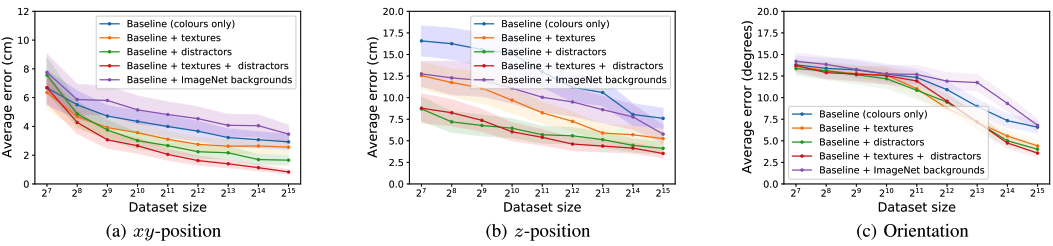
\includegraphics[height=3.7cm]{lib/graphics/influence_visual_randomness.png}
    \caption[Einfluss der Randomisierung verschiedener Effekte auf die Fehlerrate der Objekterkennung]{Einfluss der Randomisierung verschiedener Effekte auf die Fehlerrate der Objekterkennung\footnotemark}
    \label{abb:visual_randomization}
\end{figure}
\footnotetext{Enthalten in: \cite[][S. 6]{Alghonaim.5302021652021}}

Aus der Untersuchung in Abbildung sechs wird deutlich, dass die Fehleranfälligkeit der Erkennung der X-Y Position, der Z-Position und der Orientierung, durch das Hinzufügen von Texturen und Ablenkungsobjekten mitunter am besten verringert werden kann. 

\subsection{Errungenschaften unter Einsatz von Domain Randomization}

Mit dem Einsatz von DR ist es bereits nach aktuellem Stand der Forschung und Praxis ermöglicht worden, z.B. Strategien ohne reale Bilder in ausschließlich Simulationen mittelmäßiger Qualität zu trainieren und für reale Drohnenflüge im Innenbereich einzusetzen. \footcite[Vgl.][S. 1]{Sadeghi.2016} 
Weiterhin konnte erreicht werden, ausschließlich aus dem Training in Simulationen eine Objekterkennung und Lokalisation zu einer Genauigkeit von 1,5cm zu realisieren. \footcite[Vgl.][S. 1]{Tobin.2017}
Neben der Anwendung von DR zeigt die aktuelle Literatur zwar viel Forschung zu der Frage, welche Randomisierung positive Effekte erzielen kann, jedoch wenig Forschung zu detaillierten Erklärungen der Funktionsweise. \footcite[Vgl.][S. 6]{Zhao.2020}
Dies erschwert die Entwicklung effizienter Simulationen und die Bestimmung der Zufallsverteilungen zur Randomisierung. \footcite[Vgl.][S. 6]{Zhao.2020}